\documentclass[a4paper, 12pt, twoside]{article}
\renewcommand{\familydefault}{\sfdefault}
%\usepackage{helvet}
\usepackage{mathptmx}
\usepackage[a4paper, inner=30mm, outer=20mm, top=25mm, bottom=25mm]{geometry}
\usepackage[document]{ragged2e}
\usepackage{adjustbox}
\usepackage{nomencl}
\usepackage{multirow} % tabele -> merge na wierszach
\usepackage{blindtext}
\usepackage{amssymb}
\usepackage[shortlabels]{enumitem}
\usepackage{gensymb}
\usepackage{array,tabularx} %tables
\usepackage{graphicx} %zdjęcia i wykresy
\usepackage{dirtree} %drzewo katalogow
\usepackage[T1]{fontenc}
\usepackage[T1]{polski}
\usepackage[english, polish]{babel}
%\usepackage{txfonts}
\usepackage{newtxtext,newtxmath}
\usepackage{polski}
\usepackage[utf8]{inputenc}
%\usepackage{amsthm}
\usepackage{amsmath}
\usepackage{float} %do umieszczania elementow obok siebie
\frenchspacing
\DeclareUnicodeCharacter{00A0}{ } %do subfigure
\usepackage[lofdepth,lotdepth]{subfig} %macierze zdjęć
\usepackage{caption}
\usepackage[pdftex,dvipsnames]{xcolor}  % Coloured text etc.
% 
\usepackage[colorinlistoftodos,prependcaption,textsize=tiny]{todonotes} % co jeszcze zostało do zrobienia (ns Sherlock)

%\usepackage{subcaption}
\usepackage{fancyhdr}
\usepackage{pdfpages}
%\usepackage[superscript, biblabel]{cite} %cytowanie jako indeksy górne
\usepackage{float}
\captionsetup[table]{justification=raggedright,singlelinecheck=off}
\captionsetup[figure]{justification=raggedright,singlelinecheck=off}

\fancyhf{} % clear all header and footers
\renewcommand{\headrulewidth}{0pt} % remove the header rule
\renewcommand{\footrulewidth}{1pt} % remove the header rule
\fancyfoot[LE,RO]{\thepage} % Left side on Even pages; Right side on Odd pages

%bibliografia
\usepackage{csquotes}
\usepackage[backend=bibtex, style=numeric]{biblatex}
\addbibresource{bibliography/biblio.bib}


%Abbrevations
% acronyms
\usepackage{acronym} 
\usepackage{datatool}

\newcommand*{\addacronym}[2]{%
  \DTLnewrow{acronyms}%
  \DTLnewdbentry{acronyms}{Acronym}{#1}%
  \DTLnewdbentry{acronyms}{Description}{#2}%
}

% formatting
\newcommand{\tocfill}{\cleaders\hbox{$\m@th \mkern\@dotsep mu . \mkern\@dotsep mu$}\hfill}
\newcommand{\abbrlabel}[1]{\makebox[3cm][l]{\textbf{#1}\ \tocfill}}
\newenvironment{abbreviations}{\begin{list}{}{\renewcommand{\makelabel}{\abbrlabel}%
\setlength{\labelwidth}{3cm}\setlength{\leftmargin}{\labelwidth+\labelsep}%
\setlength{\itemsep}{0pt}}}{\end{list}}

%\usepackage{titlesec}
%\usepackage{titletoc}

%\titleformat{\section}
%{\normalfont\secfnt\bfseries}{\thesection}{1em}{}

\widowpenalty10000
\clubpenalty10000

\usepackage{xcolor}
\usepackage{colortbl}
\usepackage{placeins} % provides \FloatBarrier
\usepackage{tikz}
\usetikzlibrary{positioning,shapes,arrows,calc,decorations.markings,shadows}
\usepackage[hidelinks]{hyperref}


%\geometry{a4paper, left=20mm, right=20mm, top=25mm, bottom=25mm}%footskip=60pt}% don't set this manually else geometry won't know!

%%%%%%%%%%%%%%%%%%%%%%%%%%%%%%%%%%%%%%%%
\begin{document}
\emergencystretch 3em

\begin{figure}
\setlength{\voffset}{0cm}
\setlength{\hoffset}{0cm}
	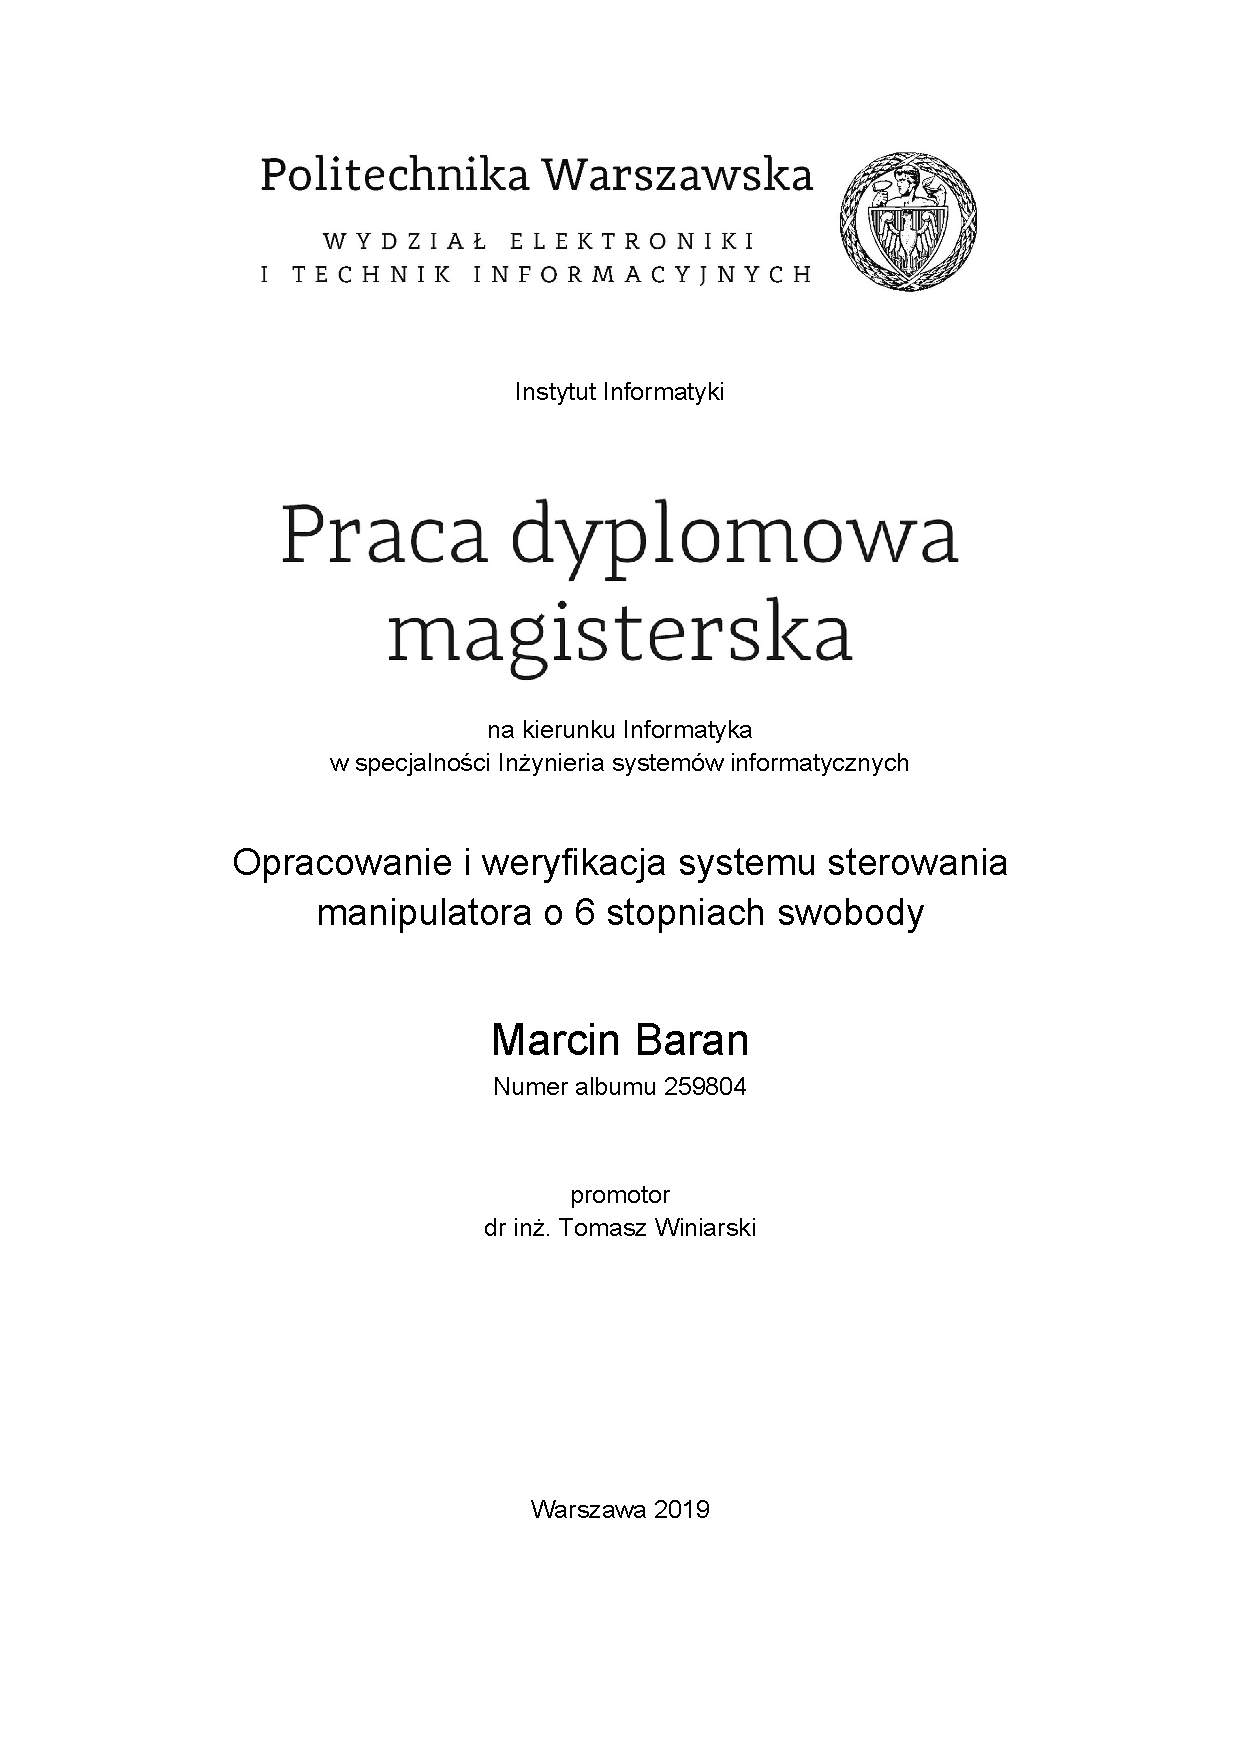
\includepdf[pages=1-2]{template/Strona_tytulowa_praca_dyplomowa_mgr_EiTI.pdf}
\setlength{\voffset}{-2.54cm}
\setlength{\hoffset}{-2.54cm}
\end{figure}
\mbox{}
\newpage
\thispagestyle{empty}
\mbox{}

%%%%%%%%%%%%%%%%%%%%%%%%%%%%%%%%%%%%%%%%
\newpage
\begin{center}
\section*{Analiza jakości sterownika manipulatora o 6 stopniach swobody}
\end{center}

\section*{Streszczenie}
\thispagestyle{empty}
\justify
W tej pracy zostaną zbadane ...
\vspace{0.5 cm}
\\
\textit{Słowa kluczowe:}
\\
\textit{Manipulator, System Czasu Rzeczywistego, Robot Operating System, }


%%%%%%%%%%%%%%%%%%%%%%%%%%%%%%%%%%%%%%%%
\newpage
\begin{center}
\section*{Quality analysis of 6 degrees of freedom robotic manipulator control driver}
\end{center}
\thispagestyle{empty}
\section*{Abstract}
\paragraph{}This thesis is focused on ...
\vspace{0.5 cm}
\\
\textit{Keywords:}
\\
\textit{Manipulator, Real Time Operating System, Robot Operating System, }

%%%%%%%%%%%%%%%%%%%%%%%%%%%%%%%%%%%%%%%%
\newpage

\includepdf[pages=1-2]{template/Oswiadczenie_autora_pracy_dyplomowej_w_jezyku_angielskim.pdf}

%%%%%%%%%%%%%%%%%%%%%%%%%%%%%%%%%%%%%%%%

\tableofcontents

%%%%%%%%%%%%%%%%%%%%%%%%%%%%%%%%%%%%%%%%
\newpage
\justify

% Początek treści	
\vspace*{1.5 cm}
\section{WPROWADZENIE}
\vspace{3.0 cm}
Systemy lotnicze w przeciągu ostatnich lat uległy znaczącemu rozwojowi. Wraz ze wzrostem osiągów statków powietrznych inżynierowie musieli dostosowywać systemy sterowania do krytycznych warunków lotu. Początkowe mechaniczne układy zostały wyparte przez elektroniczne systemy sterowania (\textit {ang. fly -- by -- wire}). Jednym z najważniejszych elementów podczas projektowania obiektów latających jest optymalizacja jego masy. W tym celu ciężkie przewody służące do wymiany informacji zastąpiono światłowodami. Współczesny samolot zawiera na swoim pokładzie wiele urządzeń elektronicznych, które wymieniają między sobą gigabajty danych na sekundę. Zapewnienie niezawodnych systemów awionicznych stało się wyzwaniem, od którego zależy bezpieczeństwo załogi i pasażerów.

Kolejny etap rozwoju systemów lotniczych skupia się na redukcji sieci przewodów w~samolocie. Bezprzewodowa wymiana danych pomiędzy urządzeniami pozwala na znaczącą oszczędność kosztów serwisowych oraz na zwiększenie masy ładownej.

Niniejsza praca poświęcona jest zagadnieniu komunikacji bezprzewodowej urządzeń awionicznych (\textit {ang. Wireless Avionics Intra -- Communication, WAIC}). Badanie tej technologii zostało przeprowadzone na podstawie autorskiego systemu wyznaczania położenia samolotu w przestrzeni ( \textit {ang. Attitude Heading Reference System, AHRS}). Na podstawie testów lotnych został wyznaczony stopień niezawodności systemu AHRS.


\vspace{1.0 cm}
\subsection{Motywacja}
Celem pracy magisterskiej jest opracowanie oraz stworzenie w pełni redundantnego systemu AHRS, stosując w nim komunikację bezprzewodową, przy wykorzystaniu gotowych urządzeń elektronicznych dostępnych na rynku (\textit {ang. Commercial -- Off -- The -- Shelf, COTS}). Zaletą tego rozwiązania jest możliwość skupienia się na tworzeniu architektury systemu, z pominięciem zagadnień związanych z wytwarzaniem dedykowanego sprzętu. 

Opracowany system znajduje zastosowanie w lotnictwie lekkim. Wyposażenie samolotów tej klasy w~dodatkowy sprzęt elektroniczny, komunikujący się przewodowo wiąże się z~modernizacją miejsca w kokpicie, które jest ograniczone. Urządzenia wykorzystujące technologię WAIC pozwalają na łatwiejszy montaż oraz nie posiadają ograniczeń związanych z~poprowadzeniem wiązki przewodów, w~ciasnej kabinie pilota. Zaprojektowany system AHRS składa się z~dwóch modułów komunikujących się bezprzewodowo. Wykorzystanie nowej technologii w~awionice posiada zarówno wiele potencjalnych zalet jak i~problemów, które nie zostały jeszcze w~pełni rozwiązane. Jednym z~nich jest wyznaczenie odpowiedniego pasma częstotliwości, które nie zakłóci pracy innych urządzeń na pokładzie samolotu oraz systemów znajdujących się w~innych samolotach w przestrzeni powietrznej. Na podstawie systemu AHRS badaniu zostanie poddane pasmo częstotliwości 2.4~GHz oraz 5~GHz w samolotach klasy lekkiej. Ponadto przebadana zostanie niezawodność redundancji systemu, która zapewnia zmianę wykorzystywanego pasma w przypadku pogorszenia jakości transmisji danych, bądź interferencji z innymi systemami.

Projekt został stworzony przy współpracy z pilotem -- Jackiem Mainką, który na potrzeby badawcze testował opracowywany system  na samolotach szkolno-treningowych de Havilland Canada DHC~--~1 Chipmunk oraz de Haviland Tiger Moth. Pozwoliło to na weryfikację poprawności systemu oraz informacji przekazywanych do pilota.

\subsection{Plan pracy}

Dokument ten stanowi raport z przeprowadzonej pracy magisterskiej. Składa się on z~następujących części:
\begin{itemize}
\item rozdział 2 zawiera wprowadzenie teoretyczne do dziedziny systemów lotniczych oraz technologi WAIC stanowiącej nowy trend w inżynierii lotniczej; zostały w nim również opisane metody wyznaczania niezawodności systemów lotniczych,
\item rozdział 3 opisuje działanie autorskiego systemu AHRS oraz budowę poszczególnych modułów systemu,
\item rozdział 4 przedstawia architekturę oprogramowania; metody przetwarzania danych wykorzystane do wyznaczania orientacji przestrzennej płatowca oraz zastosowane rozwiązania redundancji systemu,
\item rozdział 5 stanowi szczegółowy opis przeprowadzonych testów w środowisku symulacyjnym oraz podczas działania systemu w trakcie lotu płatowca,
\item rozdział 6 opisuje wyniki zebrane podczas testów; dogłębną analizę przypadków testowych oraz obliczenie niezawodności systemu AHRS,
\item rozdział 7 poświęcony jest podsumowaniu pracy.  
\end{itemize} 

%%%%%%%%%%%%%%%%%%%%%%%%%%%%%%%%%%%%%%%%
\newpage
\vspace*{1.5 cm}
\section{ANALIZA TRENDÓW}
\vspace{3.0 cm}
Zanim rozpocznie się szczegółowe studium tego, w~jaki sposób został zaprojektowany system wyznaczania położenia samolotu w przestrzeni, warto wspomnieć o~aktualnych trendach, które pojawiają się w branży lotniczej. Tworzenie niezawodnego oprogramowania, wiąże się z~dużą ilością testów, walidacji, weryfikacji oraz dokumentacji, która jest tworzona na każdym z etapów procesu. Stąd koszty produktu w~branży awionicznej związane są przede wszystkim z~zapewnieniem odpowiedniego poziomu bezpieczeństwa. W~celu tworzenia krytycznego oprogramowania stosuje się dedykowane przepisy, które opisują podejścia projektowe dla danego poziomu bezpieczeństwa (\textit{ang. Design Assurance Level, DAL}). Najważniejszym z~nich jest dokument DO~--~178C, który definiuje zasady projektowania oprogramowania, według których instytucje tj. FAA (\textit{ang. Federal Aviation Administartion}) lub ICAO (\textit{ang. International Civil Aviation Organinzation}) przeprowadzają procesy certyfikacyjne.

Przede wszystkim, ze względów bezpieczeństwa nowe narzędzia, technologie oraz metodologie, które pojawiają się w branży IT, wprowadzane są do branży lotniczej z~dużym opóźnieniem. Producenci awioniki częściej stawiają na bezpieczne rozwiązania, które zostały sprawdzone podczas wielu prób w~locie i~są niezawodne.

W niniejszym rozdziale zostaną przedstawione aktualne trendy rozwijane w~awionice, ze szczególnym uwzględnieniem technologii bezprzewodowych. W~ramach wprowadzenia w~dziedzinę niezawodności systemów zostaną opisane najpopularniejsze techniki wykorzystywane podczas wytwarzania oprogramowania.

\vspace{1.0 cm}
\subsection{Rozwój awioniki}

Ciągły postęp technologiczny w~branży IT spowodował uzależnienie niemalże każdej dziedziny od komputerów. W~podobnej sytuacji znajduje się branża lotnicza, a w szczególności awionika. Komputery odgrywają istotną rolę podczas startu oraz lądowania każdego samolotu wyposażonego w zaawansowane systemy. Jednak używanie najnowszych trendów IT w krytycznych elementach awioniki jest ryzykownym podejściem. Niemniej jednak, inżynierowie cały czas dążą do poprawy bezpieczeństwa. Osiągają to poprzez stopniowe dodawanie takich technologii jak sztuczna inteligencja, blockchain oraz komunikacja bezprzewodowa do mniej krytycznych elementów systemów.

Dzięki zwiększeniu mocy obliczeniowej komputerów oraz wykorzystaniu kart graficznych w celu zrównoleglenia obliczeń, sztuczna inteligencja w ostatnich latach zaczęła być wykorzystywana na szeroką skalę w wielu gałęziach przemysłu. Z uwagi na niedeterministyczność tego narzędzia, nie jest ono stosowane bezpośrednio w~urządzeniach awionicznych. Jednak, w~niektórych przypadkach zastosowanie sztucznej inteligencji poprawia poziom bezpieczeństwa oraz zmniejsza koszty eksploatacji. Jednym z~nich jest badanie niezawodności części mechanicznych. Każdy z~elementów lotniczych posiada maksymalny czas użytkowania, po którym daną część należy wymienić. Biorąc pod uwagę dodatkowe czynniki pogodowe, eksploatacyjne, związane ze starzeniem się elementów ten czas może się skracać, bądź wydłużać \cite{mlMechanical}. Zastosowanie metod predykcji opartych o~elementy uczenia maszynowego pozwala na dokładne oszacowanie konieczności serwisu danych elementów samolotu. Takie narzędzie umożliwia poprawę bezpieczeństwa oraz oszczędność kosztów dla linii lotniczych. Kolejne zastosowanie sztucznej inteligencji wiąże się ze zmniejszeniem błędów związanych z~czynnikiem ludzkim. Na ten rodzaj błędów najczęściej narażeni są piloci, od których zależy los pasażerów.  Firma General Electric opracowała system wspomagający pracę pilotów. Monitoruje on aktualny stan lotu, pogodę oraz czynności wykonywane przez załogę. Poprzez ciągły monitoring kokpitu, system wykrywa zmęczenie pilotów oraz inne parametry będące przyczyną błędów \cite{mlPilots}. W~przypadku wykrycia anomalii, oprogramowanie oparte o~sztuczną inteligencję informuje załogę, obsługę samolotu oraz obsługę naziemną.

Technologia blockchain, która zyskała zaufanie na~rynkach finansowych jest rozpatrywana jako narzędzie, które może wpłynąć na~poprawę bezpieczeństwa w lotnictwie. Jedną z~firm, która rozpoczęła prace w~tym kierunku jest Aeron. Eksperci zauważyli, że~kluczową przyczyną wypadków lotniczych jest zaniżanie godzin lotu, oszczędzając ogromne koszty utrzymania samolotu przez linie lotnicze \cite{aeron}. Obecnie na rynku nie istnieje znormalizowany elektroniczny system monitorowania pracy pilotów. Aby zapobiec fałszowaniu danych, zaproponowano wdrożenie technologii blockchain. Jej zadaniem byłoby gromadzenia informacji na temat lotów oraz pracy pilotów. Zapewni to większy poziom bezpieczeństwa oraz efektywniejszy przepływ informacji.

Wyposażenie samolotu ma największy wpływ na jakość oraz cenę lotu. W przypadku urządzeń awionicznych, cena utrzymania statku powietrznego może zostać zredukowana poprzez zmniejszenie masy oraz kosztów serwisowych urządzeń. Technologia komunikacji bezprzewodowej wpływa zarówno na zmniejszenie masy urządzeń danego systemu oraz na koszty serwisowe. Spośród technologii wymienionych w tym rozdziale, największy potencjał rozwojowy posiada technologia WAIC, której zastosowanie może znacząco obniżyć koszty eksploatacji. Z~tego względu stała się ona głównym tematem badań niniejszej pracy magisterskiej. Szczegółowy opis koncepcji technologii WAIC znajduje się w rozdziale \ref{waic}.


\subsection{Technologia WAIC} \label{waic}
Technologia komunikacji bezprzewodowej urządzeń awionicznych stanowi kolejny etap rozwoju lotnictwa. Nowa koncepcja ma wiele zalet oraz stwarza dodatkowe problemy, z~którymi muszą się zmierzyć inżynierowie. Główną zaletą wykorzystania WAIC jest redukcja sieci przewodów. Według danych \cite{waicDesign}, waga okablowania w helikopterze Sikorsky UH -- 60 Black Hawk jest szacowana na~około 900 kg, co stanowi 18\% jego masy startowej \cite{blackHawk}. Wykorzystanie technologii bezprzewodowej skutkuje zmniejszeniem masy, co wpływa na zmniejszenie zużycia paliwa nawet do 12\%. Ponadto proces planowania oraz rozmieszczenia wiązek elektrycznych kosztuje około 2200\$ na kilogram masy samolotu \cite{waicDesign}. Szacuje się, że każdego roku zostaje przeznaczonych około dwóch miliona roboczo -- godzin na znalezienie oraz wyeliminowaniem usterek związanych z~awarią sieci przewodów \cite{waicDesign}. 

Wraz z~pojawieniem się przemysłu internetu rzeczy (\textit{ang. Industry Internet of Things, IIoT}), rozwiązanie WAIC może być wykorzystywane do gromadzenia danych z~urządzeń awionicznych oraz ich analizie w~chmurze po zakończonym locie. Pozwala to zaoszczędzić czas i~umożliwia natychmiastowe wsparcie serwisowe w momencie wykrycia artefaktów. Temat ten jest przedmiotem badań i~rozwoju kluczowych firm w sektorze lotniczym. Jedną z~nich jest firma General Electric, która w 2017 roku wprowadziła na rynek platformę Predix -- to oprogramowania do gromadzenia i analizy danych w chmurze z maszyn przemysłowych oraz~systemów awioniki.

Jednym z~kluczowych elementów, z~którym muszą się zmierzyć inżynierowie podczas opracowywania technologii WAIC jest interferencja z~urządzeniami znajdującymi się na pokładzie samolotu, oraz z~innymi samolotami znajdującymi się w~przestrzeni powietrznej. Światowa organizacja telekomunikacyjna (\textit{ang. International Telecomunication Union, ITU}) rozważała wykorzystanie pasm 2.7~--~2.9 GHz, 4.2~--~4.4 GHz oraz 5.35~--~5.46 GHz dla technologii WAIC~\cite{itu}. Okazało się, że dla zakresu 2.7~--~2.9 GHz oraz 5.35~--~5.46 GHz istnieją niezgodności z~innymi systemami awioniki~\cite{itu}. Przyjęto, że pasmo  4.2~--~4.4~GHz nie spowoduje krytycznych w skutkach interferencji dla samolotów pasażerskich \cite{itu}, \cite{waicModulation}. Jednak, jest ono również wykorzystywane przez radiowe wysokościomierze (\textit{ang. Radio Altimeters, RAs}) na pokładzie cywilnych i~państwowych statków powietrznych. Ważne jest przeanalizowanie odpowiednich mechanizmów sprzęgania między antenami systemu WAIC i~wysokościomierzy na pokładzie samolotów. Kolejny problem stanowi określenie regulacji prawnych przez instytucje FAA oraz ICAO, w~celu użytkowania technologii bezprzewodowej w awionice. Jednym z~najważniejszych wyzwań wykorzystania tej technologii w~lotnictwie cywilnym stanowi zabezpieczenie sieci przed niepożądanymi osobami. Biorąc pod uwagę zagrożenia atakami hakerów może stanowić to jedną z~przyczyn, która będzie opóźniała wprowadzenie tej technologii na rynek.
%        \begin{figure}[hbt!]
%        \centering
%        \includegraphics[width=0.78\linewidth]{images/meteo_radar_net.png}
%        \caption{Rozmieszczenie radarów sieci POLRAD na terenie Polski.\textit{ Źródło: \cite{polradSiec}} }
%        \label{fig:meteo}
%        \end{figure}

W niniejszej pracy magisterskiej badania technologii bezprzewodowej zostały przeprowadzone na samolotach klasy lekkiej, które nie są wyposażone w~zaawansowaną awionikę. Testom została poddana bezprzewodowa sieć lokalna 802.11 b/g/n oraz 802.11 a/h/j/n/ac/ax, dla częstotliwości 2.4 GHz i 5 GHz. Zgodnie z raportem opublikowanym przez  Międzynarodowe Zrzeszenie Przewoźników Powietrznych (\textit{ang. International Air Transport Association, IATA}) częstotliwości powyżej 5 GHz są obsługiwane przez system wspomagający lądowanie MLS (\textit{ang. Microwave Landing System}) oraz radar pogodowy~\cite{iata}. Samoloty klasy lekkiej nie są wyposażone w system MLS, zatem wykorzystanie częstotliwości 5 GHz nie wpłynie na pracę tego systemu. Działanie systemu może zostać jedynie zakłócone przez interferencję z~systemem radarów meteorologicznych POLRAD, które rozmieszczone są na terenie Polski, rys.\ref{fig:meteo}. Ich częstotliwość pracy wynosi 5.42~--~5.82 GHz \cite{polrad}. W przypadku wykrycia niekorzystnych interferencji system AHRS przełączy się w~tryb redundantny i~zmieni pasmo częstotliwości komunikujących się komponentów, co poprawi jakość pracy systemu oraz przestanie zakłócać system POLRAD. Wadą przyjętego rozwiązania jest zakłócanie radaru meteorologicznego przed wejściem w~tryb redundantny. Może to spowodować chwilowe pogorszenie jakości danych meteorologicznych.

\subsection{Niezawodność systemów}

Badanie niezawodności jest kluczowym elementem podczas rozwoju systemów, od których zależy ludzkie życie. Niewielki błąd w oprogramowaniu może być katastrofalny w~skutkach. Przykładem jest system rakietowy Patriot, który 25 lutego 1991 r. zawiódł przez arytmetyczny błąd wyznaczania czasu w komputerze, przez co zginęło 28 żołnierzy a ponad 98 zostało rannych \cite{catastrophes}. Kolejnym przykładem, którego skutkiem była strata około 500 milionów dolarów był start rakiety Ariane 5. Po 37 sekundach od startu rakieta uległa autodestrukcji, spowodowanej przekroczeniem zakresu jednej ze zmiennych \cite{catastrophes}. Jak ważną rolę odgrywają testy podczas projektowania systemów awionicznych przekonali się studenci Politechniki Warszawskiej, koła naukowego awioniki MelAvio. Tworząc oprogramowanie do autorskiego autopilota dla bezzałogowych statków powietrznych nie przeprowadzili testów, związanych ze zmianą półkuli z~północnej na południową. Będąc na zawodach UAV Outback Challenge w Australii samolot rozpoczął autonomiczny lot w~kierunku przeciwnym niż został zadany. Problem związany był z~błędną interpretacją kierunków nawigacyjnych w oprogramowaniu.

Aby zmniejszyć ryzyko wystąpienia błędów katastrofalnych w skutkach, inżynierowi stosują liczne testy oraz analizy, które mają na celu wykrycie błędów na etapie projektowania. Najpopularniejsze z nich to analiza FMEA  (\textit{ang. Failure Mode and Effects Analysis}) oraz sieci Petriego, których szczegółowe opisy znajdują się w rozdziałach \ref{fmea} oraz \ref{petri}. Zastosowanie narzędzi do analizy niezawodności systemu AHRS pozwoli na wyznaczenie odpowiedniego poziomu bezpieczeństwa. Szczegółowa analiza wiarygodności projektowanego urządzenia znajduje się w rozdziale \ref{wyniki}.


%%%% Sub chapter
\subsubsection{Analiza FMEA} \label{fmea}
Koszty rozwijania systemów lotniczych zależą przede wszystkim od poziomu bezpieczeństwa jakie muszą spełniać. Im poziom krytyczności systemu jest wyższy, tym koszty związane z~weryfikacją produktu znacząco rosną. Przynależność oprogramowania systemu do danego poziomu DAL, zostaje określona na podstawie analizy funkcjonalności według normy DO~--~178C, zgodnie z tablicą~\ref{tab-dal}.

W tradycyjnym podejściu, weryfikacja produktu sprawdza czy wszystkie wymagania zostały spełnione. Odmienne podejście zaproponowała firma Honeywell. Nie polega ono na skupieniu się tylko na wymaganiach, lecz na opracowaniu także analiz systemu, które mogą sprawdzić potencjalnie wadliwe elementy \cite{honeywellFMEA}. 
\begin{table}[ht!]
\centering
\begin{tabular}{ | m{4,7cm} | m{3cm} | m{6cm} |}
\hline
    \textbf{Poziom bezpieczeństwa} & \textbf{Rodzaj awarii} & \textbf{Efekt awarii} \\ 
\hline
    \multicolumn{1}{|c|}{A} & Katastrofalny & Utrudnia poprawny lot samolotu oraz lądowanie. Ofiary śmiertelne.\\
\hline
    \multicolumn{1}{|c|}{B} & Niebezpieczny & Bardzo niski poziom bezpieczeństwa. Zwiększone obciążenie załogi. Poważne lub śmiertelne obrażenia.\\
\hline
    \multicolumn{1}{|c|}{C} & Umiarkowany & Znaczące obniżenie poziomu bezpieczeństwa. Zwiększone obciążenie załogi. Dyskomfort lub możliwe obrażenia pasażerów.\\
\hline
    \multicolumn{1}{|c|}{D} & Niewielki & Nieznaczne obniżenie bezpieczeństwa. Niewielki wzrost obciążenia załogi. Dyskomfort pasażerów. \\
\hline
\end{tabular}
\caption{Poziomy bezpieczeństwa -- DAL. \textit{ Źródło: \cite{honeywellFMEA}} }
\label{tab-dal}
\end{table}
Nowatorskie podejście inżynierowie wykorzystali w procesie projektowania systemu zarządzania komunikacją  (\textit{ang. Communications Management Function, CMF}). CMF odpowiedzialny jest za kierowanie komunikatów łącza danych między różnymi systemami na pokładzie samolotu oraz różnymi systemami naziemnymi, w tym kontrolą ruchu lotniczego (\textit{ang. Ait Traffic Control, ATC}). System został zakwalifikowany wg. standardu DO~--~178B do poziomu D. W tym poziomie, w standardowym podejściu weryfikacja systemu sprawdza jedynie wysokopoziomowe wymagania. W celu lepszej weryfikacji defektów w oprogramowaniu postanowiono wykorzystać model FMEA. To rozwiązanie pozwoliło na dokładniejszą weryfikację systemu. Nie zwiększając przy tym znacząco kosztów, co byłoby nieuniknione podczas zmiany poziomu bezpieczeństwa, z D na C.

FMEA jest to analiza możliwych rodzajów oraz przyczyn błędów pojawiających się w~oprogramowaniu. Proces składa się z~następujących etapów \cite{honeywellFMEA}:
\begin{enumerate}[1.]
   \item  \textbf{Przegląd analizy bezpieczeństwa}. Identyfikacja obszarów objętych ryzykiem wystąpienia błędów. 
   \item  \textbf{Zdefiniowanie awarii}. Określenie wszystkich potencjalnych awarii, które mogą doprowadzić do niepoprawnej pracy systemu.
   \item  \textbf{Warunki prowadzące do awarii}. Zdefiniowane sytuacji, w których dochodzi do wystąpienia anomalii systemu, warunków wejściowych oraz wyjściowych. Ocena wpływu awarii na cały system.
   \item  \textbf{Przygotowanie scenariuszy testowych}. Stworzenie przypadków testowych, które mogą odtworzyć błędną pracę systemu.
   \item  \textbf{Wykonanie oraz analiza testów}. Sprawdzenie działania systemu w krytycznych dla niego warunkach. Określenie ryzyka występowania wady oraz działań zapobiegawczych. 
\end{enumerate}
Analiza danego scenariusza testowego składa się z następujących elementów \cite{honeywellFMEA}, \cite{fmeaWiki}:
\begin{itemize}
   \item nazwa testu,
   \item opis możliwego błędu, 
   \item opis skutków błędu, 
   \item przypisanie uciążliwości błędu (\textit{ang. Severity Classification Category, SEV}) w~skali 1~--~10; krytyczne błędy powinny posiadać wyższą wartość,
   \item opis przyczyny wystąpienia danego błędu,
   \item zdefiniowanie częstotliwości występowania (\textit{ang. Occurrence Risk Category, OCC}) w~skali 1~--~10; awarie pojawiające się częściej mają wyższą wartość,
   \item opisanie procedur zapobiegających wystąpieniu danego błędu,
   \item zdefiniowanie skuteczności wykrywania  (\textit{ang. Detectability Risk Category , DRC}) w~skali 1~--~10; wada, która jest łatwiejsza w~wykryciu powinna mieć przypisaną niższą wartość,
   \item obliczenie wartości ryzyka  (\textit{ang. Risk Priority Number, RPN}); \( RPN = SEV \cdot OCC \cdot DET\).
\end{itemize}

FMEA jest narzędziem, które pozwala na ustalenie potencjalnych przyczyn oraz warunków awarii. Priorytet scenariuszy testowych jest zdefiniowany przez metrykę RPN. Im wyższa wartość tym wystąpienie danej awarii jest bardziej ryzykowne. Obliczenie wartości ryzyka jest kluczowe do określenia błędów, które powinny zostać poddane dalszym analizom. 

%%%% Sub chapter
\subsubsection{Sieci Petriego} \label{petri}
Systemy czasu rzeczywistego stały się istotnym elementem automatycznych technologii wykorzystywanych w~samochodach autonomicznych, urządzeniach medycznych czy w~lotnictwie. Proces projektowy tego typu systemów jest trudny ze względu na dużą złożoność komponentów, wymóg deterministyczności działania oraz spełnienie ograniczeń czasowych. Takie systemy muszą polegać na skutecznych metodach weryfikacji, które potwierdzą spełnienie wszystkich wymagań. Do tego celu wykorzystuje się sieci Petriego, które stanowią formalną reprezentację modelowanego systemu i~pozwalają na analizę rozproszonych komponentów.

Model klasycznej sieci Petriego jest dwukierunkowym grafem zdefiniowanym przez trzy typy obiektów: miejsca, przejścia i łuki skierowane. Łuki łączą miejsca z przejściami lub przejścia z miejscami. W~najprostszej postaci sieć Petriego może modelować zachowanie systemu podczas wystąpienia zdarzenia, definiując stany wejściowe oraz wyjściowe. W~celu zbadania dynamicznego zachowania sieci stosuje się tzw. żetony, które mogą definiować dodatkowe parametry związane z~danym miejscem podczas wystąpienia zdarzenia, może być to np. warunek prawda lub fałsz. Formalna definicja sieci składa się z 5 elementów \(N = (P,\; T,\; I,\; O,\; M_0) \)~\cite{petriIntro}:
\begin{enumerate}[(1)]
   \item \(P = \{p_1,\;p_2\;, …,\; p_m \} \) skończona liczba miejsc,
   \item \(T = \{t_1,\; t_2,\; …,\; t_n \} \) skończony zbiór przejść; \( P \cup T \neq \emptyset \) oraz \( P \cap T = \emptyset \),
   \item \(I:\; P \times T \rightarrow N \) jest to funkcja wejściowa definiująca kierunek od miejsca do przejścia; N jest nieujemną liczbą całkowitą,
   \item \(O:\; T \times P \rightarrow N \) jest to funkcja wyjściowa definiująca kierunek od przejścia do miejsca,
   \item \(M_0:\; P \rightarrow N \) jest to stan początkowy.
\end{enumerate}

Graf sieci Petriego jest strukturą w~postaci dwukierunkowego multigrafu, mającego dwa typy węzłów. Okrąg reprezentuje miejsce a prostokąt reprezentuje przejście. Ukierunkowane łuki (strzałki) łączą miejsca i przejścia. Łuk skierowany z miejsca p\textsubscript{j} do przejścia t\textsubscript{i} definiuje p\textsubscript{j} jako miejsce wejściowe do t\textsubscript{i}, oznaczone \textit{I(t\textsubscript{i}, p\textsubscript{j})} = 1. Łuk skierowany od przejścia t\textsubscript{i} do miejsca p\textsubscript{j} definiuje p\textsubscript{j} jako miejsce wyjściowe t\textsubscript{i}, oznaczane przez \textit{O(t\textsubscript{i}, p\textsubscript{j})} = 1 \cite{petriIntro}. Przykładowy graf sieci Petriego został zaprezentowany na rys. \ref{fig:petri_net}.

%        \begin{figure}[hbt!]
%        \centering
%        \includegraphics[width=0.5\linewidth]{images/petri_net.png}
%        \caption{Przykład sieci Petriego.\textit{ Źródło: \cite{petriIntro}} }
%        \label{fig:petri_net}
%        \end{figure}

Matematyczny opis przejść w grafie przedstawionym na rys. \ref{fig:petri_net} przedstawia się następująco:
\begin{itemize}[label={}, leftmargin=10.0mm]
   \item \( P = \{p_1, \; p_2,\;  p_3,\;  p_4\}\);
   \item \( T = \{t_1,\; t_2,\; t_3\} \);
   \item \( I(t_1, p_1) = 2, \;I(t_1, p_i) = 0 \) dla \( i = 2, 3, 4 \);
   \item \( O(t_1, p_2) = 2, \;O(t_1, p_3) = 1,\; O(t_1, p_i) = 0 \) dla \( i = 1, 4\);
   \item \( M_0 = (2\;0\;0\;0)^T \).
\end{itemize}

Przykład przejścia \(t_1\) został przedstawiony na rys. \ref{fig:petri_net_t1}. Stan sieci uległ zmianie i~po wykonaniu przejścia jest określony przez \(M_1 = (0\;2\;1\;0) \).

%        \begin{figure}[hbt!]
%        \centering
%        \includegraphics[width=0.47\linewidth]{images/petri_net_t1.png}
%        \caption{Przykładowa sieć Petriego po wykonaniu przejścia t\textsubscript{1}.\textit{ Źródło: \cite{petriIntro}} }
%        \label{fig:petri_net_t1}
%        \end{figure}

Jako narzędzie matematyczne, sieci Petriego pozwalają projektantowi systemu na wnikliwą analizę oraz identyfikację właściwości funkcjonalnych, specyficznych dla domeny danej aplikacji. Bazowanie na standardowych grafach sieci Petriego, zaprezentowanych na rys.  \ref{fig:petri_net} oraz  \ref{fig:petri_net_t1} może być niewystarczające, do modelowania rozbudowanych systemów czasu rzeczywistego. Dla bardziej wymagających modeli stosuje się wysokopoziomowe sieci Petriego, które dodatkowo wprowadzają rozróżnialność żetonów oraz zależności czasowe. Wysokopoziomowe sieci to: kolorowe sieci Petriego  (\textit{ang. Colored Petri Net, CPN}), czasowe sieci Petriego (\textit{ang. Timed Petri Net, TPN}), w~których wyróżnia się sieć deterministyczną (\textit{ang. Deterministic Timed Petri Net, DTPN}) oraz stochastyczną (\textit{ang. Stochastic Timed Petri Nets, STPN})  \cite{petriIntro}.

Sieć CPN charakteryzuje to, że każdy żeton przynależy do danego koloru, co określa jego przynależność do danej grupy. Ponadto każde miejsce oraz przejście posiada dołączony zestaw kolorów. Podczas wykonywania przejść żetony są umieszczane w wyjściowym miejscu analogicznie jak w podstawowej sieci Petriego. Z~tą różnicą, że zmianie ulegają jedynie żetony o~kolorze, który jest określony w~danym miejscu oraz w~zadanym przejściu \cite{petriIntro}.

Kolejny rodzaj sieci -- TPN charakteryzuje się wykorzystaniem zmiennych, określających zależności czasowe. Sieć deterministyczna -- DTPN wykonuje przejścia co określony kwant czasu. Składa się ona z~tych samych elementów co zwykła sieć, lecz dodatkowo zawiera parametr  \( \tau: \; T \rightarrow R^+\), który jest funkcją przejścia w~deterministycznej dziedzinie czasu. Sieci STPN wykonują przejścia bazując na losowym prawdopodobieństwie. Czasowo wykładnicze, stochastyczne sieci Petriego zwane są SPN (\textit{ang. Stochastic Petri Nets}). Składają się one z~tych samych elementów co standardowa sieć, lecz dodatkowo zawierają parametr \( \Lambda: \; T \rightarrow R\). Określa on szybkość wykładniczego indywidualnego rozkładu czasu przejść \cite{petriIntro}. 

Sieci Petriego, które rozważają wpływ czasu podczas analiz, są jedną z najpopularniejszych metod wykorzystywanych do opisu systemów czasu rzeczywistego. Analizując sieci TPN projektant ma możliwość określenia dostępności danego systemu w dziedzinie czasu. Ocenie podlega przepływ informacji pomiędzy modułami oraz czy system jest w stanie przetworzyć określoną ilość zadań, zdefiniowaną w wymaganiach. Mając takie dane możliwe jest wyznaczenie poziomu wiarygodności systemu. Przykład wykorzystania sieci SPN w modelowaniu urządzeń awionicznych został opisany w rozdziale \ref{hmfm}.

%%%% Sub chapter
\subsubsection{Zarządzanie błędami w awionice} \label{hmfm}
Pomimo wszelkich starań inżynierów, stworzenie urządzeń, które będą działać bezbłędnie jest zadaniem bardzo trudnym. Nawet najlepiej opracowane systemy mogą być ofiarą czynników losowych, tj. promieniowanie kosmiczne, które może spowodować wystąpienie zjawiska SEU (\textit{ang. Single Event Upset}) i wprowadzić urządzenie w stan nieokreślony. Aby przeciwdziałać takiemu zjawisku w systemach awionicznych wprowadza się moduły monitorowania (\textit{ang. Health Monitoring, HM}) oraz zarządzania błędami (\textit{ang. Fault Management, FM}).

Przykład zastosowania modułów HM/FM, które zostały oparte o~stochastyczne sieci SPN został zaprezentowany przez chińskich naukowców, dla koncepcji zintegrowanej awioniki (\textit{ang. Integrated Modular Avionics, IMA}) \cite{stochasticHMFMPetri}. Podejście do tworzenia urządzeń w modelu IMA zakłada odejście od tradycyjnego modelu tworzenia odrębnej aplikacji dla każdego systemu, lecz tworzenie systemu, który wspiera różne rodzaje aplikacji. Dzięki takiemu rozwiązaniu wzrasta oszczędność masowa poprzez redukcję wielu podsystemów. Wprowadzenie modułów monitorowania oraz zarządzania błędami ma na celu zapewnienie wiarygodności, że system jest zdolny do prawidłowego działania nawet w przypadku wystąpienia błędów. Moduł HM jest odpowiedzialny za monitorowanie, identyfikację, lokalizację błędu oraz zgłoszenie go do modułu FM. W~przypadku zgłoszenia awarii aktywowany jest moduł zarządzania błędami, którego zadaniem jest podjęcie odpowiedniej akcji mającej na celu przywrócenie poprawnej funkcjonalności systemu. Moduł monitorowania systemu odpytuje cyklicznie moduły na temat ich aktualnego stanu. W~przypadku wykrycia anomalii procedura zapewnia aktywowanie systemu FM.

Wykorzystanie stochastycznych sieci Petriego w warstwie HM/FM umożliwia tworzenie zintegrowanego modelu, weryfikującego działanie systemu w dziedzinie czasu. Ponadto daje możliwość podzielenia systemu na warstwy i analizowanie ich wpływu na cały model~\cite{stochasticHMFMPetri}. Takie podejście zastosowali inżynierowie z Beijing dzieląc system na niezależne warstwy, gdzie każda z nich składa się ze współpracujących modeli HM oraz FM \cite{stochasticHMFMPetri}. 

Moduł odpowiedzialny za monitorowanie błędów został podzielony na trzy części, przedstawione na rys. \ref{fig:hm_spn}. Część CQ (\textit{ang. Current Layer Query}) odpowiedzialna jest za sprawdzanie stanu obiektów w losowych odstępach czasu. Podczas sprawdzania obiektu, po wywołaniu przejścia \textit{Timer\_C} zostaje wykonane przejście \textit{Query\_C} i bezpośredni powrót do stanu \textit{Idle}, gdy nie występują żadne anomalie. W przypadku, gdy zostaje wykryty błąd aktywowany jest moduł FM poprzez przejście \textit{Activate\_FM1}, strzałka 3 wskazuje na obsługę błędu. Raport z~przechwyconego błędu zostaje zlokalizowany w~przejściu \textit{Sub\_Report}. Moduł RP (\textit{ang. Reply}) odbiera zapytania od warstwy nadrzędnej, zbiera informacje i~odsyła je do warstwy odpytującej. Ostatnia część SQ (\textit{ang. Subordinate Layer QUery}) jest wykorzystywana przy ścisłej współpracy z~pozostałymi warstwami systemu. Cyklicznie wysyła zapytania (strzałka 5) do innych warstw i~po otrzymaniu pozytywnych odpowiedzi (strzałka 6) powraca do stanu \textit{Idle}, w~przeciwnym razie następuje obsługa błędu.
%        \begin{figure}[hbt!]
%        \centering
%        \includegraphics[width=0.94\linewidth]{images/hm_spn.png}
%        \caption{Opis modelu HM za pomocą sieci SPN.\textit{ Źródło: \cite{stochasticHMFMPetri}} }
%        \label{fig:hm_spn}
%        \end{figure}  

Moduł odpowiedzialny za zarządzanie błędami został przedstawiony na rys. \ref{fig:fm_spn}. Składa się on wielu mniejszych modułów, z~których każdy jest odpowiedzialny za obsługę określonego błędu. Każda akcja naprawcza kończy się stanem pozytywnym lub negatywnym. Rezultaty działania modułu FM są kolekcjonowane w \textit{Error\_Report\_Pool} i~przesyłane do modułu HM.
%        \begin{figure}[hbt!]
%        \centering
%        \includegraphics[width=0.81\linewidth]{images/fm_spn.png}
%        \caption{Opis modelu FM za pomocą sieci SPN.\textit{ Źródło: \cite{stochasticHMFMPetri}} }
%        \label{fig:fm_spn}
%        \end{figure}

Komunikacja między warstwami jest specyfiką danego systemu. Stosuje się rozwiązania, które zakładają, że moduły zarządzania błędami mogą odnosić się do pozostałych warstw w~przypadku negatywnej obsługi danej anomalii. Zostało to przedstawione na przykładzie części SQ modułu HM.

Zaprezentowany model wykorzystania sieci Petriego w~urządzeniach IMA znajduje zastosowanie w~przypadku badania technologii WAIC w~systemie AHRS. Moduły monitorowania oraz zarządzania błędami posiadają duży potencjał do zarządzania komunikacją bezprzewodową. 
Wykorzystanie analizy FMEA oraz sieci SPN umożliwia przeprowadzenie procesu weryfikacji systemu. Skorzystanie z~tych narzędzi pozwala na wstępną analizę problemu oraz sporządzenie modelu obsługi błędów. Wynikiem tego procesu jest wyznaczenie metryk związanych z~oszacowaniem średniego czasu naprawy systemu, dostępności systemu oraz prawdopodobieństwem wystąpienia awarii.



%%%%%%%%%%%%%%%%%%%%%%%%%%%%%%%%%%%%%%%%
\newpage
\vspace*{1.5 cm}
\section{SYSTEM AHRS}
\vspace{3.0 cm}

\vspace{1.0 cm}
\subsection{Zasada działania}
TO DO
\subsection{Redundancja}
TO DO

\subsection{Mechanika}
TO DO

\subsubsection{Moduł pilota}
TO DO

\subsubsection{Moduł akwizycji danych}
TO DO

\subsection{Elektronika}
TO DO
\subsubsection{Moduł pilota}
TO DO

\subsubsection{Moduł akwizycji danych}
TO DO

\subsection{Oprogramowanie}
TO DO

\subsubsection{Moduł pilota}
TO DO

\subsubsection{Moduł akwizycji danych}
TO DO 


%%%%%%%%%%%%%%%%%%%%%%%%%%%%%%%%%%%%%%%%
\newpage
\vspace*{1.5 cm}
\section{ARCHITEKTURA OPROGRAMOWANIA}
\vspace{3.0 cm}

\vspace{1.0 cm}

\subsection{Struktura projektu}
TO DO

\subsection{Wykorzystane narzędzia}
TO DO

\subsection{Moduł pilota}
TO DO

\subsubsection{Struktura oprogramowania}
TO DO

\subsubsection{Interfejs użytkownika}
TO DO
\subsubsection{Komunikacja}
TO DO

\subsection{Moduł akwizycji danych}
TO DO
\subsubsection{Struktura oprogramowania}
TO DO
\subsubsection{Kąty orientacji przestrzennej}
TO DO
\subsubsection{Odbiornik GPS}
TO DO
\subsubsection{System uzgadniający}
TO DO

\subsection{Redundancja oprogramowania}
TO DO

\subsubsection{Zakłócenia SEU}
TO DO

\subsubsection{Watchdog}
TO DO

\subsubsection{Oprogramowanie symulacyjne}
TO DO



%%%%%%%%%%%%%%%%%%%%%%%%%%%%%%%%%%%%%%%%
\newpage
\vspace*{1.5 cm}
\section{TESTY}
\vspace{3.0 cm}

\vspace{1.0 cm}
\subsection{Symulacje}
TO DO

\subsection{Testy w locie}
TO DO

\subsection{Podsumowanie}


%%%%%%%%%%%%%%%%%%%%%%%%%%%%%%%%%%%%%%%%
\newpage
\vspace*{1.5 cm}
\section{OPRACOWANIE WYNIKÓW}  \label{wyniki}
\vspace{3.0 cm}

\vspace{1.0 cm}
\subsection{Analiza FMEA}
TO DO

\subsection{Sieć Petriego}
TO DO

\subsection{Analiza bezpieczeństwa}
TO DO

\subsection{Wiarygodność technologii WAIC}
TO DO 

%%%%%%%%%%%%%%%%%%%%%%%%%%%%%%%%%%%%%%%%
\newpage
\vspace*{1.5 cm}
\section{PODSUMOWANIE}
\vspace{3.0 cm}

%%%%%%%%%%%%%%%%%%%%%%%%%%%%%%%%%%%%%%%%
\newpage
\section*{DODATEK A. Zawartość płyty CD}
\addcontentsline{toc}{section}{DODATEK A. ZAWARTOŚĆ PŁYTY CD}
\vspace{3.0 cm}

%%%%%%%%%%%%%%%%%%%%%%%%%%%%%%%%%%%%%%%%
\newpage
% Bibliografia
\section*{}
\addcontentsline{toc}{section}{BIBLIOGRAFIA}
\printbibliography

%%%%%%%%%%%%%%%%%%%%%%%%%%%%%%%%%%%%%%%%
\newpage
\section*{Wykaz symboli i skrótów}
\addcontentsline{toc}{section}{WYKAZ SYMBOLI I SKRÓTÓW}

\DTLnewdb{acronyms}
\addacronym{WAIC}{Wireless Avionics Intra–Communication}
\addacronym{AHRS}{Attitude Heading Reference System}
\addacronym{COTS}{Commercial–Off–The–Shelf}
\addacronym{DAL}{Design Assurance Level}
\addacronym{FAA}{Federal Aviation Administartion}
\addacronym{ICAO}{International Civil Aviation Organinzation}
\addacronym{IIoT}{Industry Internet of Things}
\addacronym{RAs}{Radio Altimeters}
\addacronym{ITU}{International Telecomunication Union}
\addacronym{FMEA}{Failure Mode and Effects Analysis}
\addacronym{CPN}{Colored Petri Net}
\addacronym{SPN}{Stochastic Petri Nets}
\addacronym{TPN}{Timed Petri Net}
\addacronym{DTPN}{Deterministic Timed Petri Net}
\addacronym{STPN's}{Stochastic Timed Petri Nets}
\addacronym{SEU}{Single Event Upset}
\addacronym{HM}{Health Monitoring}
\addacronym{FM}{Fault Management}
\addacronym{IMA}{Integrated Modular Avionics}

% Sort the database
\DTLsort*{Acronym}{acronyms}

%Show acronyms
\begin{itemize}[label={}, leftmargin=*]
\DTLforeach*{acronyms}{\thisAcronym=Acronym,\thisDesc=Description}
   {\item \textbf{\thisAcronym}   \thisDesc}
\end{itemize}

%%%%%%%%%%%%%%%%%%%%%%%%%%%%%%%%%%%%%%%%
\newpage
\addcontentsline{toc}{section}{SPIS RYSUNKÓW}
\listoffigures

%%%%%%%%%%%%%%%%%%%%%%%%%%%%%%%%%%%%%%%%
\newpage
\addcontentsline{toc}{section}{SPIS TABLIC}
\listoftables
\end{document}